\documentclass[a4paper,12pt]{article}

\usepackage{graphicx} % Required for inserting images
\usepackage{amsmath,amssymb,amsfonts}
\usepackage{subcaption}
% Use Times New Roman font
\usepackage{times}
\usepackage[a4paper, top=1in, bottom=0.8in, left=1.1in, right=0.8in]{geometry}
\usepackage{float}
\usepackage{listings}
\usepackage{xcolor} % For customizing code colors
\setlength{\parindent}{0pt}
\usepackage{titlesec} % Add this to your preamble
\titleformat{\section}
{\normalfont\large\bfseries}{\thesection}{1em}{}
% Set spacing for sections
\titlespacing*{\section}
{0pt}  % Left spacing
{1ex} % Space before (adjust this value)
{0.5ex}  % Space after (adjust this value)

\begin{document}
\section{Experiment No. 3}


\section{Experiment Title }
External characteristic curve of self-excited DC Generator.
\section{Objective}
	The objectives of this lab are as follows:
\begin{itemize}
	\item To determine the relationship between terminal voltage \( V_T \) and load current \( I_L \) as the load is applied and varied.
	\item To investigate the factors contributing to the drop in terminal voltage when the generator is loaded.
	\item To identify the breakdown point on the characteristic curve.
	
\end{itemize}


\section{Theory}

The external characteristic curve of a self-excited DC generator represents the relationship between its terminal voltage \( V_T \) and load current \( I_L \). It is observed that when a self-excited shunt generator is loaded, its terminal voltage \( V \) drops with an increase in load current. This drop in voltage is undesirable, especially when the generator is supplying current for light and power. In such applications, it is essential that \( V \) remains practically constant and independent of the load. This condition of constant voltage is almost impossible to achieve with a shunt generator unless the field current is automatically adjusted by a regulator. Without such regulation, the terminal voltage drops significantly as the load on the generator increases.



\begin{figure}[H]
	\centering
	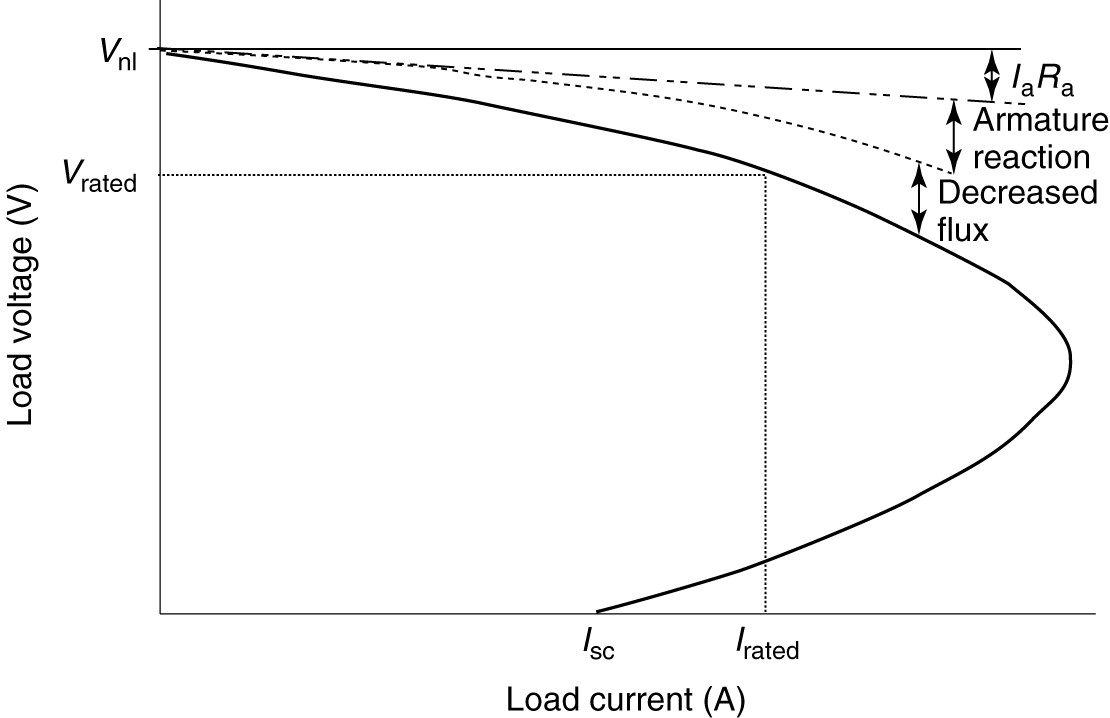
\includegraphics[width=0.5\linewidth]{Images/4}
	\caption{Characteristic curve of Self-excited DC Generator}
	\label{fig:volt-amp-characteristic-of-a-self-excited-dc-generator}
\end{figure}
There are three main reasons for the drop in terminal voltage of a shunt generator under load conditions:
\begin{enumerate}
	\item \textbf{Armature Resistance Drop:} \\
	As the load current increases, more and more voltage is consumed in overcoming the ohmic resistance of the armature circuit. Hence, the terminal voltage is given by:
	\[
	V = E - I_a R_a
	\]
	where:
	\begin{itemize}
		\item \( V \) is the terminal voltage,
		\item \( E \) is the induced e.m.f. in the armature under load condition,
		\item \( I_a \) is the armature current, and
		\item \( R_a \) is the armature resistance.
	\end{itemize}
	
	\item \textbf{Armature Reaction Drop:} \\
As the load current increases, more and more voltage is consumed in the ohmic resistance of the
armature circuit. Hence, the terminal voltage 	\[
V_T = E_g - I_a R_a
\] is decreased where E is the induced e.m.f.
in the armature under load condition.
	
	\item \textbf{Armature reaction drop:} \\
Due to the demagnetising effect of armature reaction, pole flux is weakened and so the induced
e.m.f. in the armature is decreased.
\item \textbf{Reduction in Field Current:}	The drop in terminal voltage V due to 1. and 2. results in a decreased field current $I_f$ which
	further reduces the induced e.m.f.
\end{enumerate}
\section{Required Apparatus}
\begin{enumerate}
	\item Variable Resistor (Ratings: Resistance: 5000$\Omega$, Current: 0.31A),
	\item Variable Resistor (Ratings: Resistance: $2\times 200$$\Omega$, Current: 1.58A),
	\item Variable Resistor (Ratings: Resistance: 50$\Omega$, Current: 3.16A),
	\item Three Phase Power Supply (Ratings: Voltage: 400V, Current: 10A),
	\item Three Phase Power Supply (Ratings: Voltage: 400V, Current: 10A),	
\item DC Multimeter (Ratings: Voltage: 600V, Current: 20A) 
\item Three Phase Asynchronous Motor (Ratings: Power: 500W, Voltage: 400V/230V, Current: 1.8A/1.3A, Speed: 1380 rpm),
\item DC Generator (Ratings: Power: 300W, Voltage: 220V, Current: 1.4A)
\item Tacho-Generator (Ratings: Current: 0.07A max, Speed: 5000 rpm max).
\end{enumerate}
\section{Circuit Diagram}
\begin{figure}[H]
	\centering
	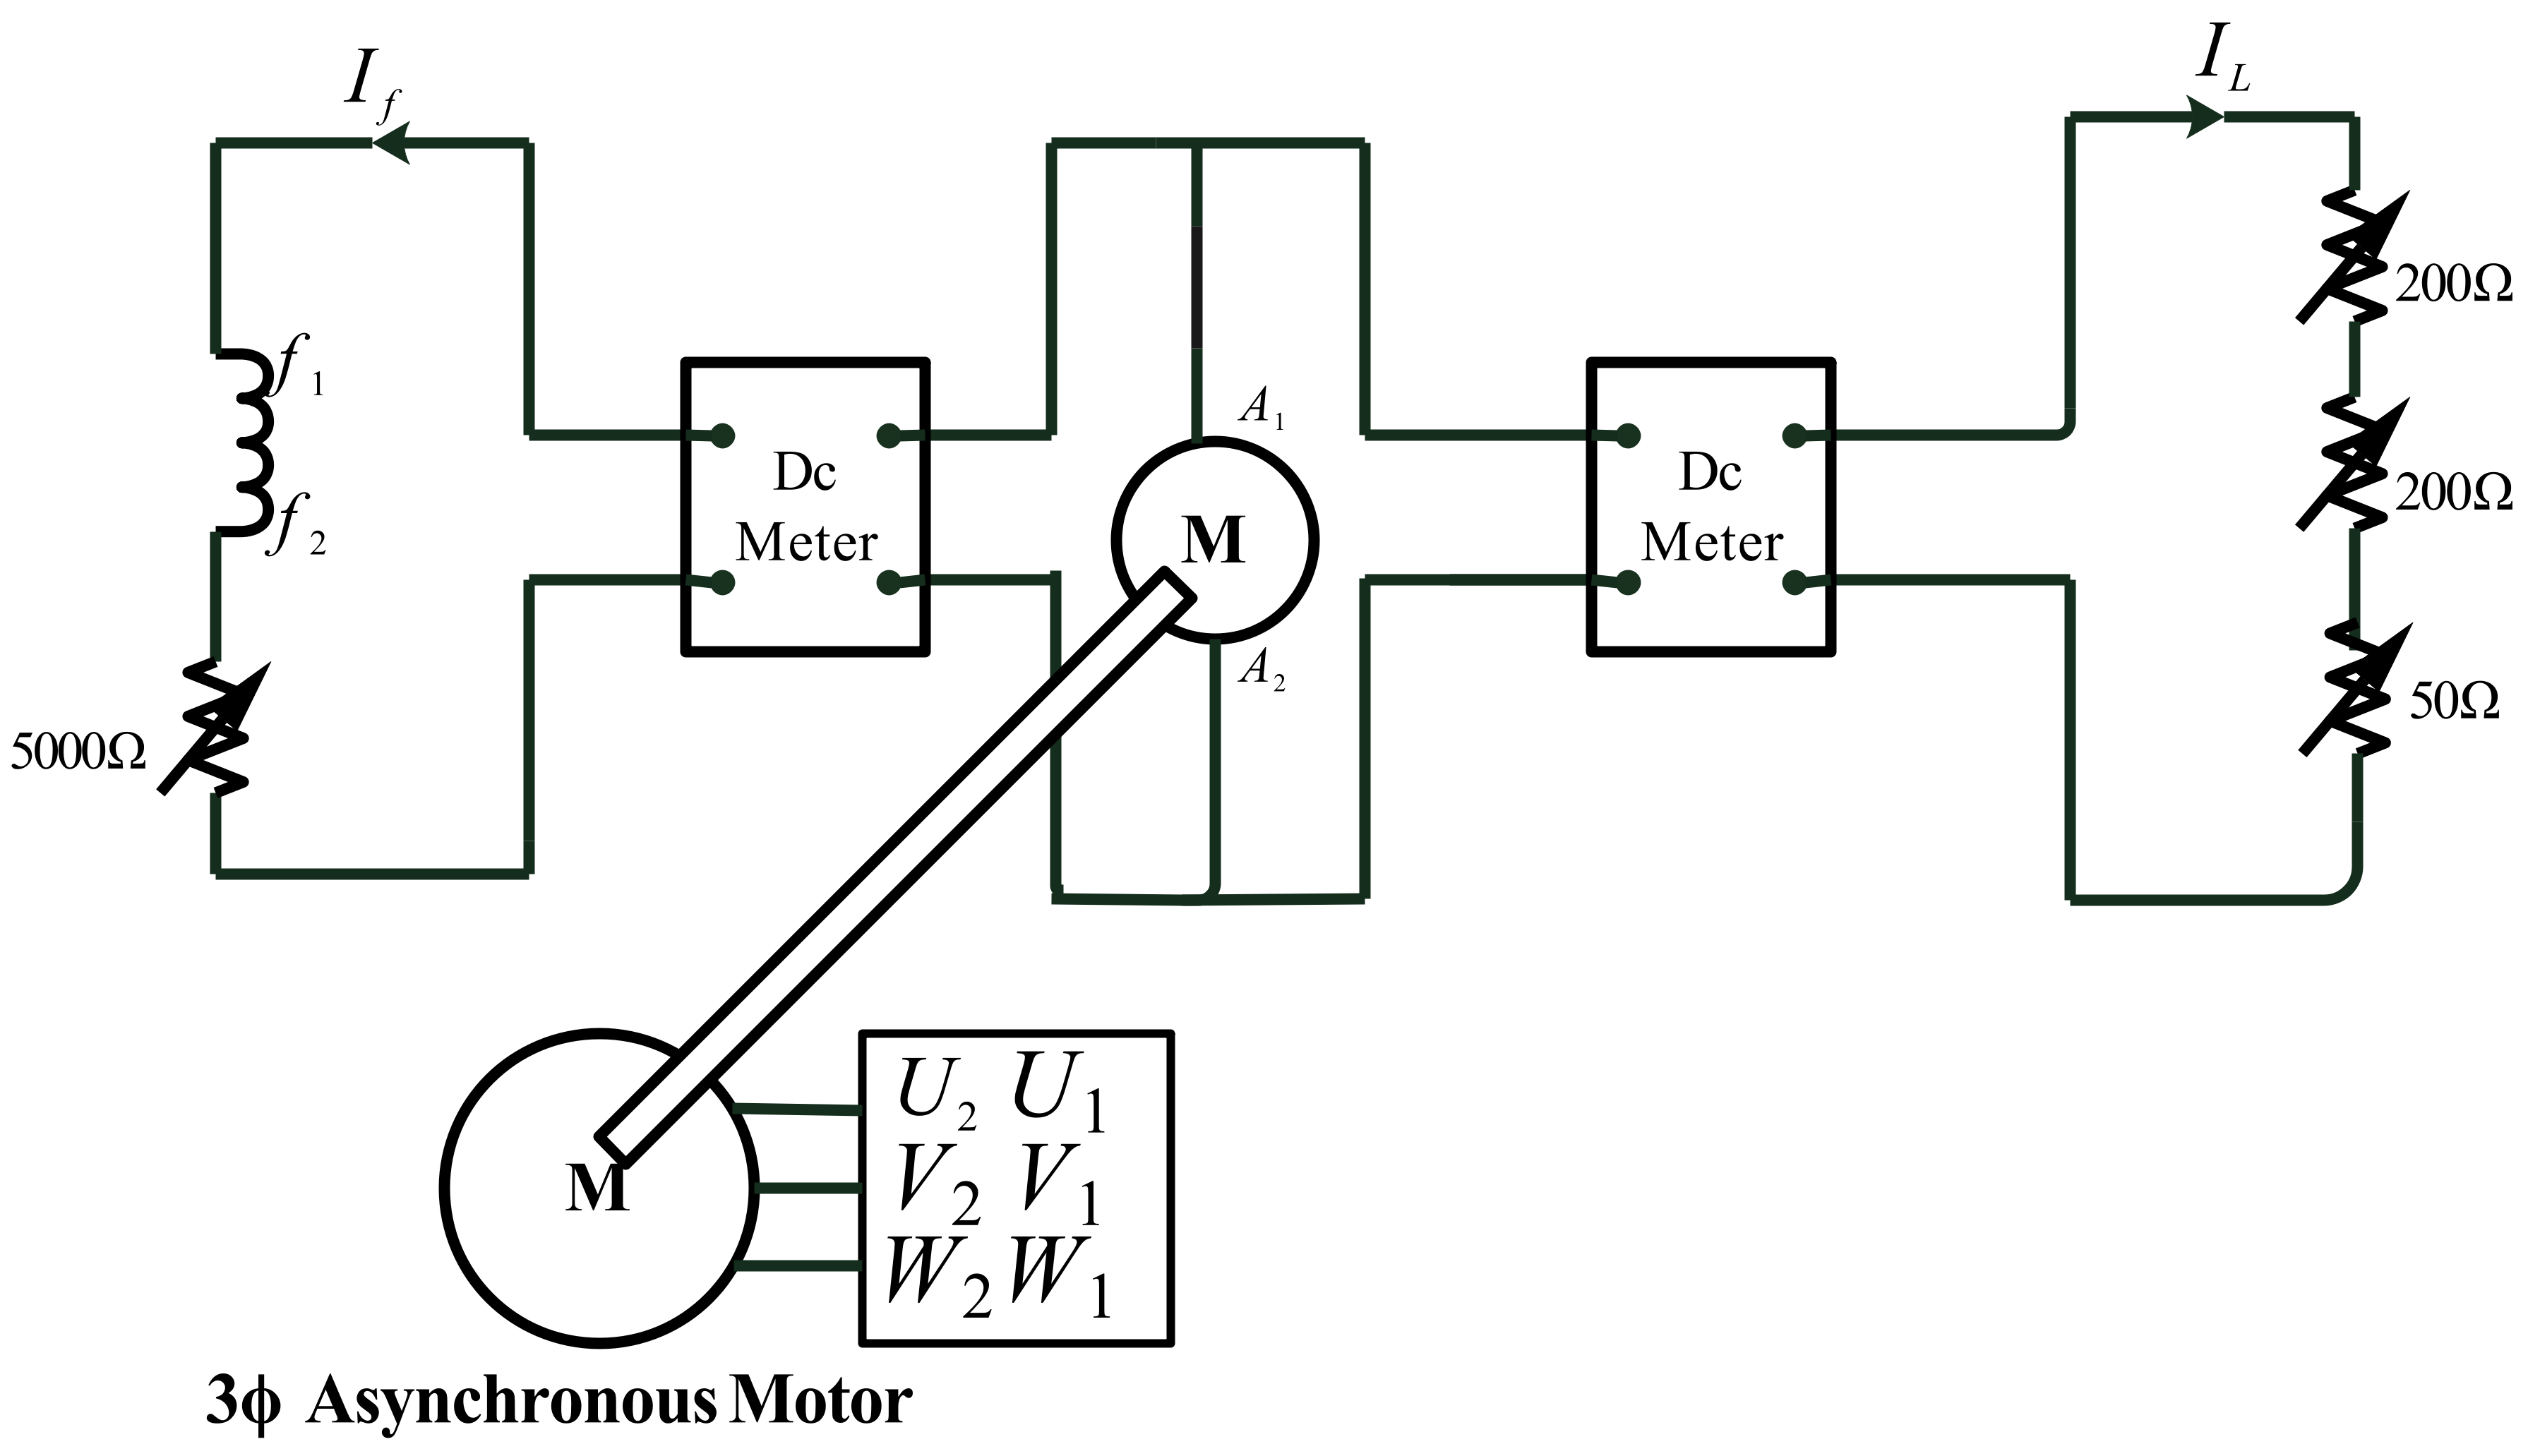
\includegraphics[width=0.76\linewidth]{Images/3}
	\caption{Circuit Diagram for self-excited DC Generator}
	\label{fig:2}
\end{figure}





\newpage
\section{Data Table}
\begin{table}[H]
		\centering
	\caption{Readings of Load Current ($I_L$), Terminal Voltage ($V_T$) and Field Current ($I_f$)}
		\scalebox{0.80}{
	\begin{tabular}{|c|c|c|c|}
		\hline
		\textbf{\begin{tabular}[c]{@{}c@{}}SI\\ No.\end{tabular}} & \textbf{\begin{tabular}[c]{@{}c@{}}Load Current\\ $I_L$\\ (A)\end{tabular}} & \textbf{\begin{tabular}[c]{@{}c@{}}Terminal Voltage\\ $V_T$\\(V)\end{tabular}} & \textbf{\begin{tabular}[c]{@{}c@{}}Field Current\\ $I_f$\\ (A)\end{tabular}} \\ \hline
		1.                                                        & 0.000                                                                 & 220                                                                       & 0.079                                                                  \\ \hline
		2.                                                        & 0.424                                                                 & 204                                                                       & 0.07                                                                   \\ \hline
		3.                                                        & 0.445                                                                 & 202.74                                                                    & 0.075                                                                  \\ \hline
		4.                                                        & 0.484                                                                 & 198.6                                                                     & 0.075                                                                  \\ \hline
		5.                                                        & 0.540                                                                 & 194.6                                                                     & 0.071                                                                  \\ \hline
		6.                                                        & 0.600                                                                 & 189.3                                                                     & 0.070                                                                  \\ \hline
		7.                                                        & 0.647                                                                 & 185.5                                                                     & 0.068                                                                  \\ \hline
		8.                                                        & 0.707                                                                 & 180                                                                       & 0.065                                                                  \\ \hline
		9.                                                        & 0.787                                                                 & 170                                                                       & 0.063                                                                  \\ \hline
		10.                                                       & 0.828                                                                 & 161.4                                                                     & 0.058                                                                  \\ \hline
		11.                                                       & 0.865                                                                 & 156.0                                                                     & 0.057                                                                  \\ \hline
		12.                                                       & 0.896                                                                 & 145.8                                                                     & 0.052                                                                  \\ \hline
		13.                                                       & 0.940                                                                 & 139.2                                                                     & 0.050                                                                  \\ \hline
		14.                                                       & 0.958                                                                 & 133.1                                                                     & 0.048                                                                  \\ \hline
		15.                                                       & 0.962                                                                 & 130.3                                                                     & 0.047                                                                  \\ \hline
		16.                                                       & 0.971                                                                 & 128.8                                                                     & 0.045                                                                  \\ \hline
		17.                                                       & 0.973                                                                 & 126.3                                                                     & 0.044                                                                  \\ \hline
		18.                                                       & 0.990                                                                 & 122.9                                                                     & 0.042                                                                  \\ \hline
		19.                                                       & 1.012                                                                 & 118.5                                                                     & 0.040                                                                  \\ \hline
		20.                                                       & 1.024                                                                 & 114.2                                                                     & 0.040                                                                  \\ \hline
		21.                                                       & 1.045                                                                 & 110.6                                                                     & 0.00                                                                   \\ \hline
		22.                                                       & 1.093                                                                 & 105.6                                                                     & 0.00                                                                   \\ \hline
		23.& 1.100                                                                 & 99.6                                                                      & 0.00                                                                   \\ \hline
	\end{tabular}
}
\end{table}	
\section{Graph}
\begin{figure}[H]
	\centering
	\includegraphics[width=0.72\linewidth]{"D:/DOWNLOAD 2024 V2/LATEX FILE/EEE_2208/EXP03_EEE2208/Images/1"}
	\caption{Terminal Voltage $(V_T)$ vs. Load Current $(I_L)$ characteristic curve}
	\label{fig:1}
\end{figure}
\section{Discussion}



In this experiment, the external characteristic curve of the self-excited DC generator was analyzed to understand its performance under various load conditions. The readings for terminal voltage \( V_T \) and load current \( I_L \) were recorded as the load resistance was gradually decreased.\\
It was observed that as the load resistance was lowered, the load current increased, resulting in a slight drop in terminal voltage. This behavior was consistent with Ohm's law, where the relationship between voltage, current, and resistance was expected. However, as the load current approached higher levels, significant voltage drops were noted, indicating the limitations of the generator's capacity to maintain a constant output.\\
The breakdown point of the characteristic curve was reached when the generator delivered current levels significantly above its normal operating range. Beyond this point, attempts to decrease load resistance resulted in decreased load current, contrary to the expected outcome. This unusual behavior was attributed to the severe armature reaction, which caused a drastic reduction in terminal voltage, overshadowing the effects of resistance changes.



\end{document}